\chapter{Text-guided Transient Attribute Transfer}\label{zero-shot}

In the previous chapter, I discussed appearance manipulation at the image level through the proposal of a low-level editing framework. The retouching framework is designed to enhance photographs by editing intricate details while refining high-level features, such as lighting or content. Conversely, this chapter focuses on a high-level manipulation task known as transient attribute transfer. In this task, we observe varying changes to the scene, including relighting, content addition or removal, and more. These edits are still learned implicitly without decomposing images into the 3D scene components.

The appearance of a scene can change dramatically over the course of a day or across seasons. While main elements, such as buildings, lakes, or forests generally remain the same, we often notice illumination changes that alter the appearance of the scene’s contents. Additionally, we might observe content being added or removed between seasons or throughout the day. For example, a scene may be covered with snow in a transient attribute change from "summer" to "winter". These changes are difficult to estimate implicitly due to the entanglement of content, illumination, and reflectance. In this chapter, I explore a conditional generative model for transferring transient attributes based on a target attribute. Specifically, I use variants of pre-trained latent diffusion models conditioned with text prompts indicating the target attribute.

I first fine-tune a stable diffusion model using the v1.5 checkpoint weights \cite{rombach2022high} and ControlNet \cite{zhang2023adding} on the Transient Attribute Dataset \cite{laffont2014transient} of 8,571 images. However, I observe that these highly complex models can easily overfit to a small dataset even in a fine-tuning setting. This challenge leads me to explore a zero-shot setup that does not require an additional dataset and use these pre-trained foundation models as a prior to guide the desired transfer instead. I evaluate the mentioned techniques qualitatively on the test images from the Transient Attribute Dataset \cite{laffont2014transient} . The zero-shot approach effectively transfers the attributes while preserving high-level content.

\section{Introduction}\label{sec:zero-shot-intro}


Attributes are high-level descriptions of visual concepts. In contrast to categories, which broadly classify objects or scenes based on high-level features, attributes often remain continuous or variable, changing across instances of the same category. For instance, in the "outdoor scene" category, attributes can be associated with seasonal transitions (e.g., winter to spring), weather changes (e.g., rainy, sunny), or times of day (e.g., daylight, sunset, night). In this work, I focus on such transient attributes that dynamically shape the visual appearance of an outdoor scene.


\begin{figure}[ht]
  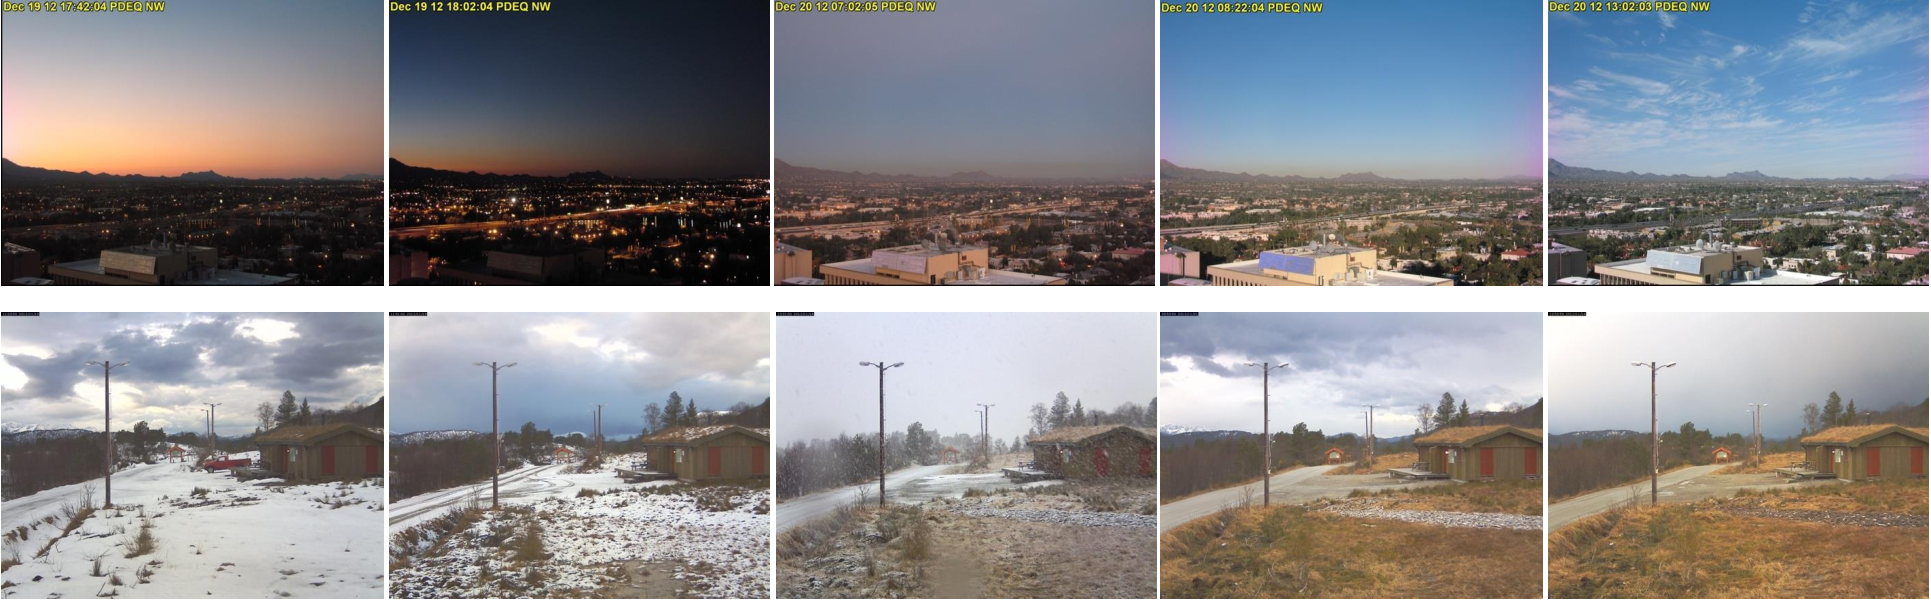
\includegraphics[width=\textwidth]{Chapters/zero-shot-tat-figs/tat-teaser.pdf}
  \caption{Transition of the illumination throughout the day or the weather changes across seasons alter the scene appearance significantly in terms of colour, tone, texture, and style. However, main content, such as the structure, permanent objects, etc. remains unchanged. Transient attribute transfer aims to capture alterations related to such temporal effects. Images from the Transient Attribute Dataset \cite{laffont2014transient}.}
  \label{fig:zero-shot-teaser}
\end{figure}

Transient attributes influence our perception of a scene by altering appearance-related properties, such as colour, texture, and overall atmosphere, i.e., style and tone. From the slow transition of sunrise to daylight, the accumulation of snow on the ground, to the clearing sky after an overcast day, these attributes define the dynamic and captivating nature of the visual world. Recent works in the fields of computer vision and graphics have engaged with the transfer of such attributes, either under the umbrella term of high-level image editing or as standalone tasks. Capturing such temporal changes plays a crucial role in a range of applications, such as photography, filmmaking, gaming, and virtual and augmented reality, for producing photorealistic simulations. However, the accurate transfer of transient attributes is highly challenging due to the requirement for a deep understanding of the scene components as well as the need to maintain essential content.

This chapter aims to address these challenges by exploring recent advancements in generative models, more specifically diffusion-based approaches. The observation that fine-tuning these foundation models with a small dataset can lead to overfitting motivates me to leverage the pre-trained models to guide the transfer process in a way that improves generalisability. Therefore, I focus on a zero-shot approach that eliminates the need for extensive additional datasets, instead utilising the robust priors embedded in foundation models. I evaluate this approach through qualitative comparisons with fine-tuned models and demonstrate its ability to effectively capture transfers, such as seasonal changes and varying lighting and weather conditions, while preserving the scene's core features.

%By advancing the understanding and manipulation of transient scene attributes, this research contributes to the broader goal of enhancing the realism and flexibility of visual content generation, paving the way for more immersive and contextually adaptive visual experiences.

In summary, this chapter contributes to the broader goal of manipulating appearance in a data-efficient manner by:

%Multiple Transformation Blending
\begin{itemize}

   \item Exploiting a pre-trained diffusion model in a zero-shot setting, requiring only an input image and a single-word text prompt describing the target attribute.
    
   \item Capturing the ever-changing transitions in an outdoor scene without any explicit decomposition of scene components.

\end{itemize}


\section{Related work}\label{zero-shot-RW}
This work falls into the broader category of text-guided image-to-image translation. Here, I will review the related works on text-guided image generation and manipulation.

\subsection{Text-to-image synthesis}

Recent years have seen significant advancements in text-to-image synthesis, from the initial Generative Adversarial Network (\gls{GAN})-based approaches \cite{li2020manigan,xu2018attngan,zhang2017stackgan,zhang2018stackgan++} to the latest diffusion \cite{gu2022vector,ho2020denoising,nichol2021improved,ramesh2022hierarchical,rombach2022high,saharia2022photorealistic,song2020denoising,zhang2023adding} and transformer models \cite{ding2022cogview2,esser2021taming,ramesh2021zero,yu2022scaling}. Notably, DALL·E 2 \cite{ramesh2022hierarchical} and Imagen \cite{ho2022imagen} condition the diffusion models with text prompts. Pre-trained CLIP models \cite{radford2021learning} are also explored for guidance in image generation with text descriptions \cite{crowson2022vqgan,ramesh2022hierarchical}. More recently, Stable Diffusion \cite{rombach2022high}, trained on a large number of image-text pairs \cite{schuhmann2021laion}, was released to the public and has since become a key tool in the field for both image generation and manipulation. Later, ControlNet \cite{zhang2023adding} includes spatial conditioning controls, such as edges, depth, segmentation, and human pose, to Stable Diffusion for image generation with enhanced control. Our work utilises the latest advancements in conditional image generation and explores their pre-trained capacity to transfer transient attributes.


\subsection{Text-guided image manipulation}
Pre-trained generator models and CLIP \cite{radford2021learning} have been deployed for text-guided image manipulation, with extended applications including video editing and style transfer \cite{bar2022text2live,gal2022stylegan,kwon2022clipstyler,liu2021fusedream,patashnik2021styleclip}. For instance, StyleCLIP \cite{patashnik2021styleclip}, based on a \gls{GAN}-based generative model StyleGAN \cite{karras2020analyzing}, modifies input latent vectors with a CLIP-based loss, while VQGAN-CLIP \cite{crowson2022vqgan} guides VQ-GAN \cite{esser2021taming} using CLIP for high-quality image generation and editing. Furthermore, diffusion models have been extensively studied for text-driven image manipulation \cite{avrahami2022blended,gal2022image,kawar2023imagic,kim2022diffusionclip,liu2023more,meng2021sdedit,nichol2021glide,ruiz2023dreambooth}. Imagic \cite{kawar2023imagic} obtains text embeddings that align with the input image and the target text prompt and finetunes a pre-trained diffusion model to capture the desired edits. InstructPix2Pix \cite{brooks2023instructpix2pix} finetunes Stable Diffusion \cite{rombach2022high} with human instructions generated with the help of GPT-3 \cite{brown2020language}.

Similar to our work, DiffEdit \cite{couairon2022diffedit}, MasaCtrl \cite{cao2023masactrl}, and ZeCon \cite{yang2023zero} perform tuning-free text-guided image manipulation without requiring additional extensive datasets. DiffEdit \cite{couairon2022diffedit} utilises DDIM inversion \cite{dhariwal2021diffusion,song2020denoising} along with automatically generated masks to capture local image edits. MasaCtrl \cite{cao2023masactrl} introduces a mutual self-attention method guided by a mask that is extracted from cross-attention maps in diffusion models. ZeCon \cite{yang2023zero} introduces a zero-shot contrastive loss that works in a patch-based feature space for image style transfer. DiffEdit \cite{couairon2022diffedit} and MasaCtrl \cite{cao2023masactrl} aim for local edits with mask guidance, potentially missing global transfers that are more dominant in the transitions between transient attributes. ZeCon \cite{yang2023zero} edits high-level content without concerns about photorealism, consequently not preserving the main structures. In contrast, I explore a tuning-free method that can 1) maintain photorealism and the essential content, and 2) capture global transfers, such as illumination changes, without any mask guidance.




\section{Methodology}
I first finetune two pre-trained models,  a stable diffusion model with the v1.5 checkpoint weights \cite{rombach2022high} and ControlNet \cite{zhang2023adding} on the Transient Attribute Dataset \cite{laffont2014transient}. 

\subsection{Transient attribute dataset} 

The dataset consists of 8,571 images captured from 101 webcams, all annotated with 40 attribute labels. In order to capture static viewpoints over long periods, \citeauthor{laffont2014transient} \cite{laffont2014transient} chose a group of outdoor webcams from the following existing sources: the Archive of Many Outdoor Scenes \cite{jacobs2007consistent} and the Webcam Clip Art Dataset \cite{lalonde2009webcam}. The dataset includes images of scenes with large variations, ranging from mountainous views to urban areas, with resolutions varying between $640 \times 360$ and $4,000 \times 3,000$. Images captured from the same webcam are also manually aligned to a reference frame using a warping method.

\paragraph{Attribute labels.} Attributes are selected through crowdsourcing from an initial list of 92 scene attributes. In a crowdsourced experiment on Amazon Mechanical Turk, \citeauthor{laffont2014transient} \cite{laffont2014transient} observe that some properties rarely occur or do not vary across scenes, while weather-, lighting-, or emotion-related properties can change dramatically across the images of the same scene. This leads to a reduced number of attributes (40) in five categories: lighting, weather, seasons, subjective impressions, and additional attributes.

The attributes are as follows: \textit{dirty, daylight, night, sunrise sunset, dawn dusk, sunny, clouds, fog, storm,snow
, warm, cold, busy, beautiful, flowers, spring, summer, autumn, winter, glowing, colourful, dull, rugged, midday, dark
, bright, dry, moist, windy, rain, ice, cluttered, soothing, stressful, exciting, sentimental, mysterious, boring, gloomy, lush}.

Each image is later annotated with the corresponding attributes by workers on Amazon Mechanical Turk. As attributes lie on a continuous spectrum, the workers are asked to respond with "totally / a little / not at all" to the question "how much does each image exhibit this attribute?" These responses are later assigned label values of 1 / 0.5 / 0, and aggregated scores ranging from 0 (attribute not present) to 1 (attribute present) are estimated using a two-stage estimator. More details about the workers' performance and the estimation approach can be found in Section 3.2 of the main paper \cite{laffont2014transient}.

\subsection{Transient attribute transfer}

\paragraph{Finetuning.} Following the same convention for the attributes list, I select the annotations with scores > 0.8 to generate the associated text prompts for the images. In cases where images have multiple annotations with high scores, I merge them with a comma separator. For example, if an image has high scores for both the "sunny" and "daylight" annotations, then the text prompt is "daylight, sunny". I finetune the models with 8,571 images conditioned on the text prompts (attribute labels). For the finetuning of the models, I reform the dataset following the instructions provided in the models' official GitHub repository. I only finetune the U-Net parameters, freezing the parameters of all other components (encoders and decoders).

\begin{figure}[ht]
  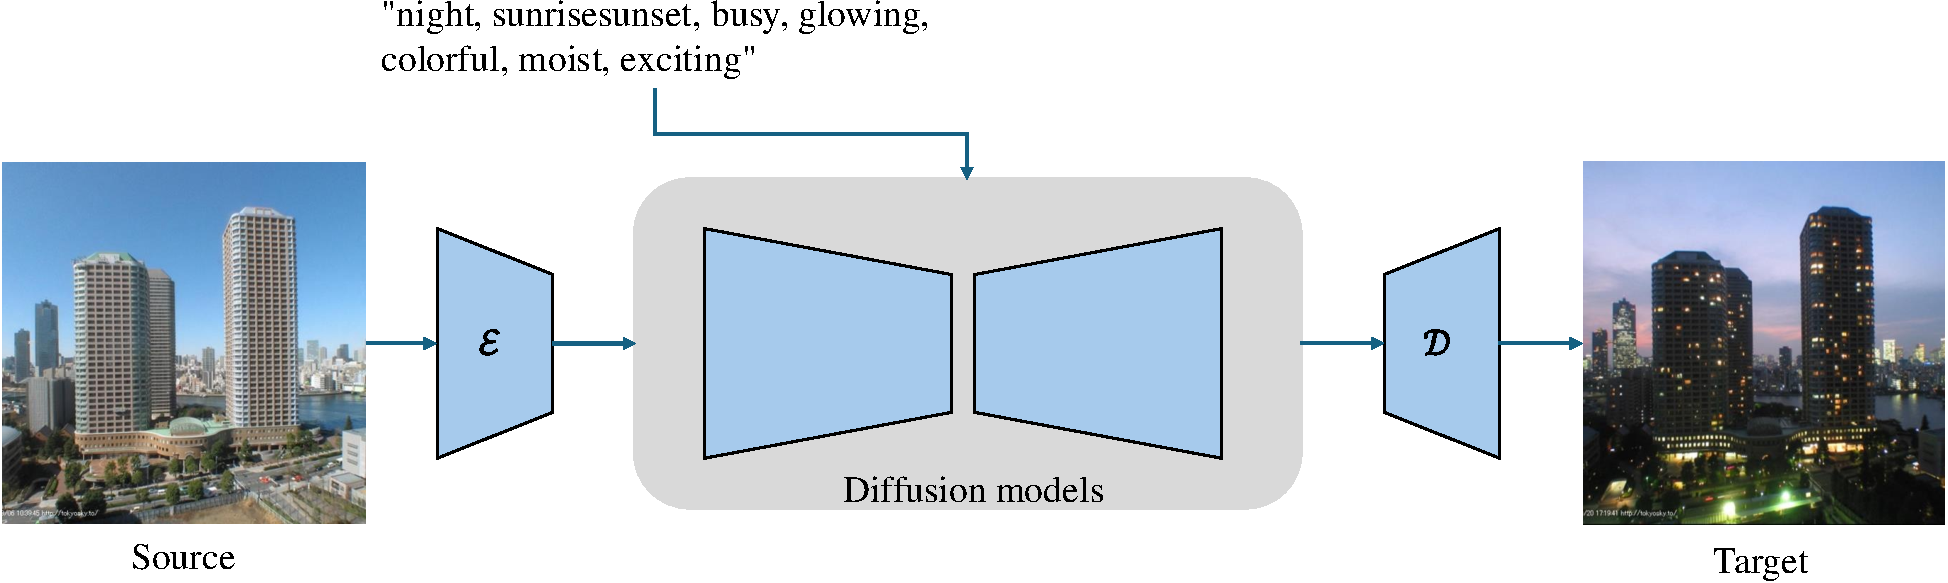
\includegraphics[width=\textwidth]{Chapters/zero-shot-tat-figs/TAT-overview.pdf}
  \caption{The fine-tuning of both Stable Diffusion v1.5 and ControlNet includes an input image (source) along with a text prompt extracted from the annotations with the objective of learning the target attribute. Note that the figure only consists of a representative of the diffusion models. The network architecture of ControlNet remains the same as described in the main paper \cite{zhang2023adding}.}
  \label{fig:finetuning-overview}
\end{figure}


%\TODO{GPU info and how long you trained}

%\TODO{explain DDIM and DDPM in background}

\paragraph{DDIM inversion.} To guide the input image with a latent diffusion model, I utilise \gls{DDIM} inversion \cite{dhariwal2021diffusion,song2020denoising} , which inverts the DDIM sampling process by adding noise to the input image. Here, the idea is to start the sampling process from the noisy input image instead of pure random noise. Figure \ref{fig:ddim-inversion} shows that the input image gradually turns into random noise as the number of time steps increases. Instead of using the random noise generated at the last step, if I start from, let’s say, somewhere in the middle, I can preserve the main structures of the input image, for example, third subfigure in Figure  \ref{fig:ddim-inversion}). Later, while sampling an output image with this intermediate latent, the priors embedded in the pre-trained model can steer the noisy input image towards a target image with the text guidance.

\begin{figure}[ht]
  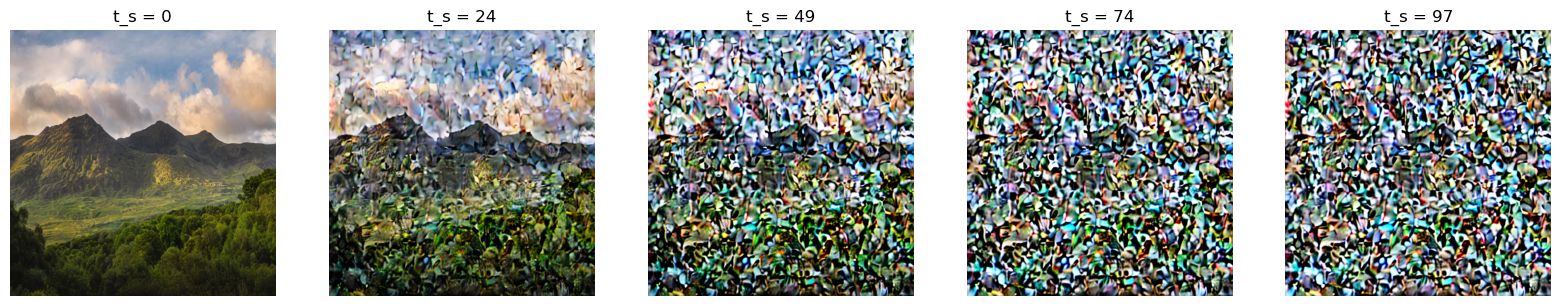
\includegraphics[width=\textwidth]{Chapters/zero-shot-tat-figs/DDIM_forward.png}
  \caption{In the forward process of a diffusion model, an input image gradually turns into a random noise by adding small amounts of Gaussian noise at each time step. Here, the total number of time steps is 100. In DDIM inversion, the sampling process replaces the random noise with an intermediate time step, such as $t_s = 49$, for its starting point.}
  \label{fig:ddim-inversion}
\end{figure}

Note that I use a latent diffusion model; hence, the noising process indeed occurs in the latent space. Here, I decode the noised latents with the VAE decoder of the model for visualisation. 

\paragraph{DDIM sampling.}
At a given time step $t$, the noisy image $\bm{x}_t$ is the original image ($\bm{x}_0$) mixed with some noise ($\epsilon$), mathematically defined as follows (from the DDIM paper \cite{song2020denoising}):

\begin{equation}
\bm{x}_t = \sqrt{\alpha_t}\bm{x}_0 + \sqrt{1 - \alpha_t}\epsilon
\end{equation}
where $\epsilon$ is some gaussian noise with unit variance, $\alpha_t$ is the noise scheduler. 

Sampling starts with pure noise at time step $T$ and gradually approaches $t = 0$. The next $\bm{x}_{t-1}$ in the sampling trajectory is calculated by predicting the noise $\epsilon_{\theta}(\bm{x}_t)$ with the learned model, which is used to predict $\bm{x}_0$. The noise prediction is incorporated into the "step" towards $\bm{x}_t$. Additional noise can also by added with a scale $\sigma_t$:

\begin{equation}
\bm{x}_{t -1} = \sqrt{\alpha_{t - 1}}\biggl(\frac{\bm{x}_t - \sqrt{1 - \alpha_t}\epsilon_{\theta}^{(t)}(\bm{x}_t)}{\sqrt{\alpha_t}}\biggl) + \sqrt{1 - \alpha_{t - 1} - \sigma_t^2} \, . \, \epsilon_{\theta}^{(t)}(\bm{x}_t) + \sigma_t \, \epsilon_t
\label{eq:ddim-sample}
\end{equation}
Here, the first term inside the parenthesis is the "predicted $\bm{x}_0$" multiplied with the noise scheduler, and the second term is the "direction pointing to $\bm{x}_t$". In my experiments, I do not add any additional noise term ($\sigma_t = 0$) to keep the sampling process fully deterministic. That is, samples follow a fixed procedure from $\bm{x}_T$ to $\bm{x}_0$.

Another important term to mention before discussing the experimental results is the guidance scale. A pre-trained U-Net model predicts the noise $\epsilon_t$ at each time step. In the text-conditional case, the noise prediction includes one term for the unconditional prediction and one for the text-conditioned prediction. The output noise prediction becomes the weighted average of these two, with a guidance scale $\sigma_s$:

$$\epsilon_{pred} = \epsilon_{uncond} + \sigma_s * (\epsilon_{text} - \epsilon_{uncond} )$$.

Here, I work with the classifier-free guidance.

%here: \href{https://github.com/lllyasviel/ControlNet}{ControlNet}, \href{https://github.com/timothybrooks/instruct-pix2pix}{Stable Diffusion v1.5}. 


\section{Experiments}\label{zero-shot-exp}

\subsection{Finetuning}
During finetuning, ControlNet learns a highly accurate mapping between the input and target images according to text guidance. Figure  \ref{fig:controlnet-train} shows that even the details, such as tree branches, small buildings, or windows, remain as they should. The effect of text guidance is also clearly visible in the model outputs, such as "daylight" enlightening the scene (first two columns) or "night" darkening the street (right-most column).
 
\begin{figure}[ht]
  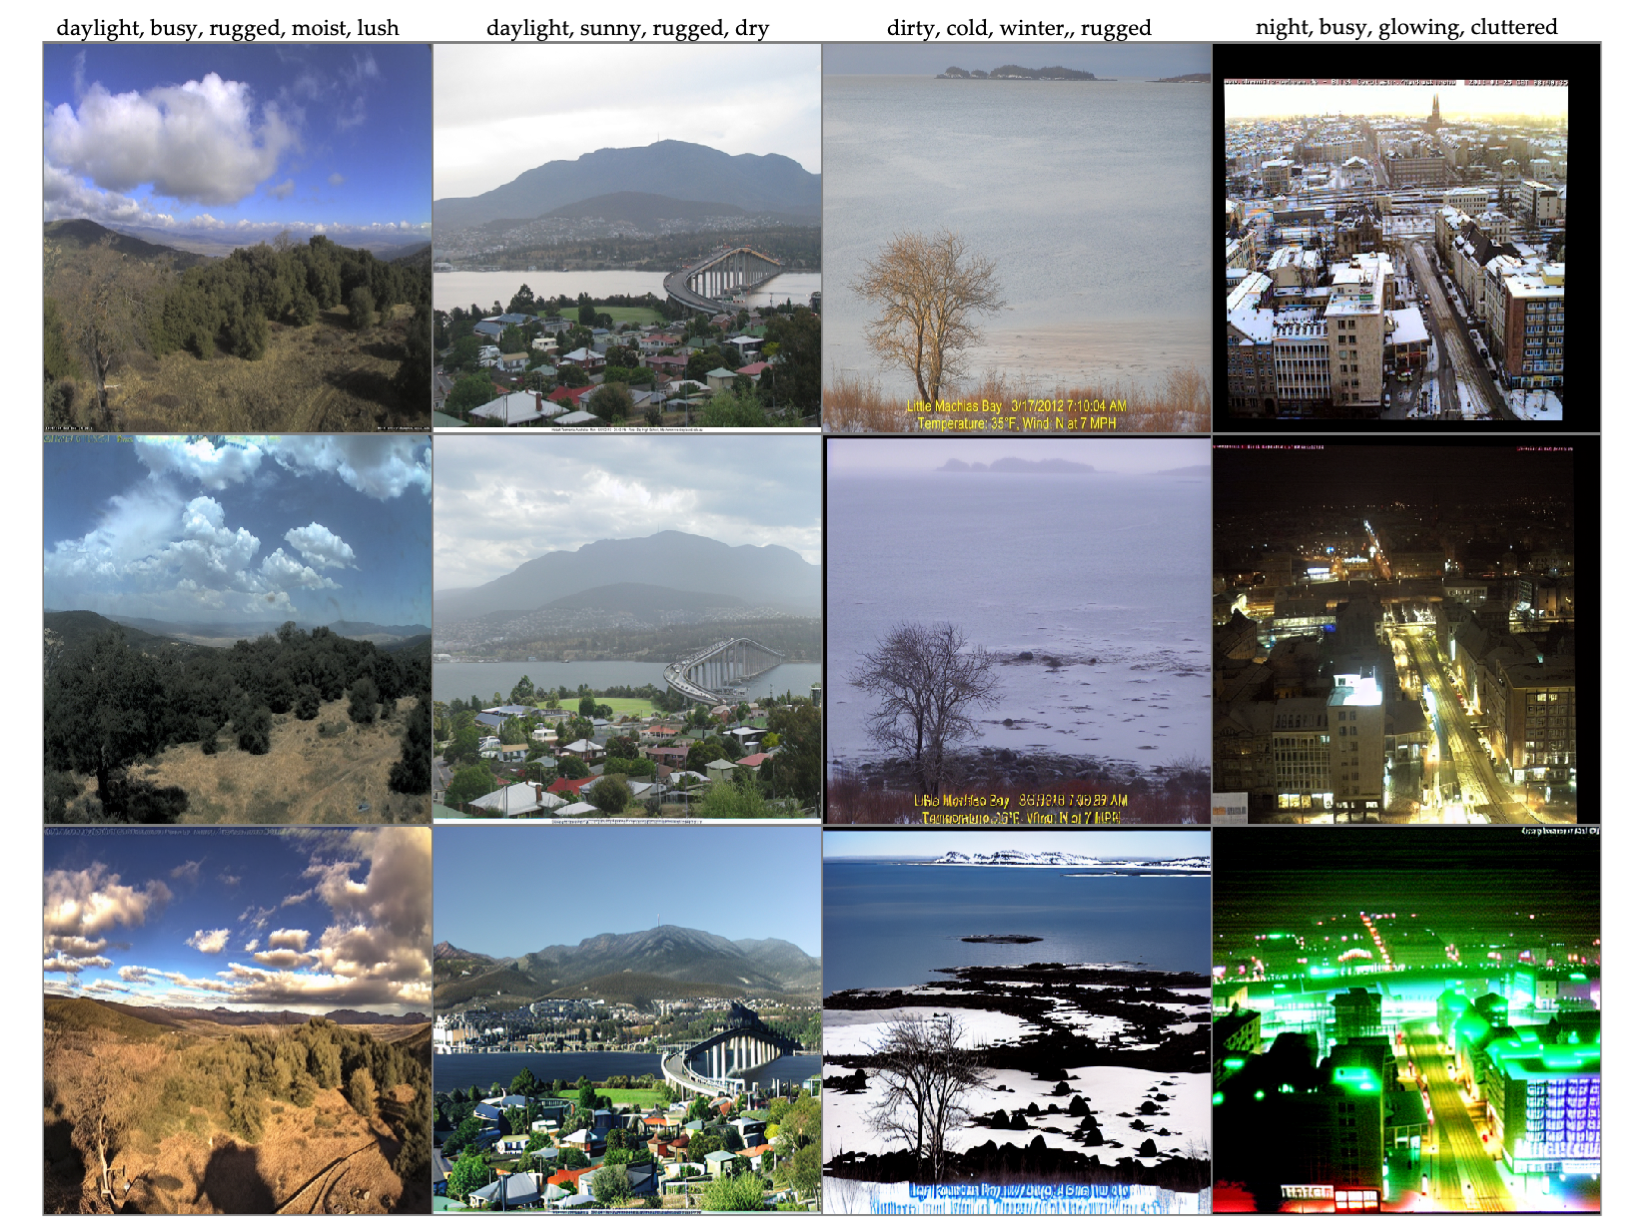
\includegraphics[width=\textwidth]{Chapters/zero-shot-tat-figs/Controlnet2.png}
  \caption{ControlNet samples from the training examples guided with the associated text prompts. Rows demonstrate input images, target images and the model outputs, in order. The subtitles indicate the attributes guiding the model.}
  \label{fig:controlnet-train}
\end{figure}

Although ControlNet performs extremely well on the training examples, its complex architecture, with a significantly high number of parameters, causes overfitting to the dataset of approximately 8000 images, leading to a performance decrease on the test dataset with losses in details and structures (Figure \ref{fig:zero-shot-comparison} - third right-most column). For instance, the car and the hut in the second row from the bottom appear to have been replaced with an unfinished construction. Another example would be the "night" prompt, where additional buildings are placed in what was supposed to be the parking area.

In terms of overfitting, the finetuned Stable Diffusion (second right-most column in Figure \ref{fig:zero-shot-comparison}) can preserve the wooden house in the "winter" prompt and maintain the car structure in "daylight." It can also perform content creation with respect to text guidance, comparable to ControlNet. However, both models can overdo the content creation with some newly added structures, such as clouds, covering large areas in the input image.

\subsection{Zero-shot latent diffusion}
In the zero-shot case, the similarity of the model output to the input image is controlled by the start step  $t_s$, which counts from the end step  $T$. That is, the input of the sampling process is the intermediate latent that was denoised for $t_s$ steps, starting with pure noise. I keep the total number of steps as 150 in all experiments. I also experimented with larger and smaller time steps; however, I observed that as long as the ratio of the start step to the total number of steps is the same, the results remain similar. Therefore, I only experimented with the start step to maintain the core features.


The guidance scale is another crucial parameter for the success of the zero-shot setting, as it transforms the input image according to the desired attribute. I tried four different values (10, 20, 30, 40) and observed that there is no one-size-fits-all value for all images. This also applies to the start step and poses a trade-off between the preservation of the essential content and the strength of the desired transfers. I chose the zero-shot results in Figure \ref{fig:zero-shot-comparison}  (right-most column) based on the subjective judgement of this trade-off.

\subsection{Grid search}

\begin{figure}[ht]
  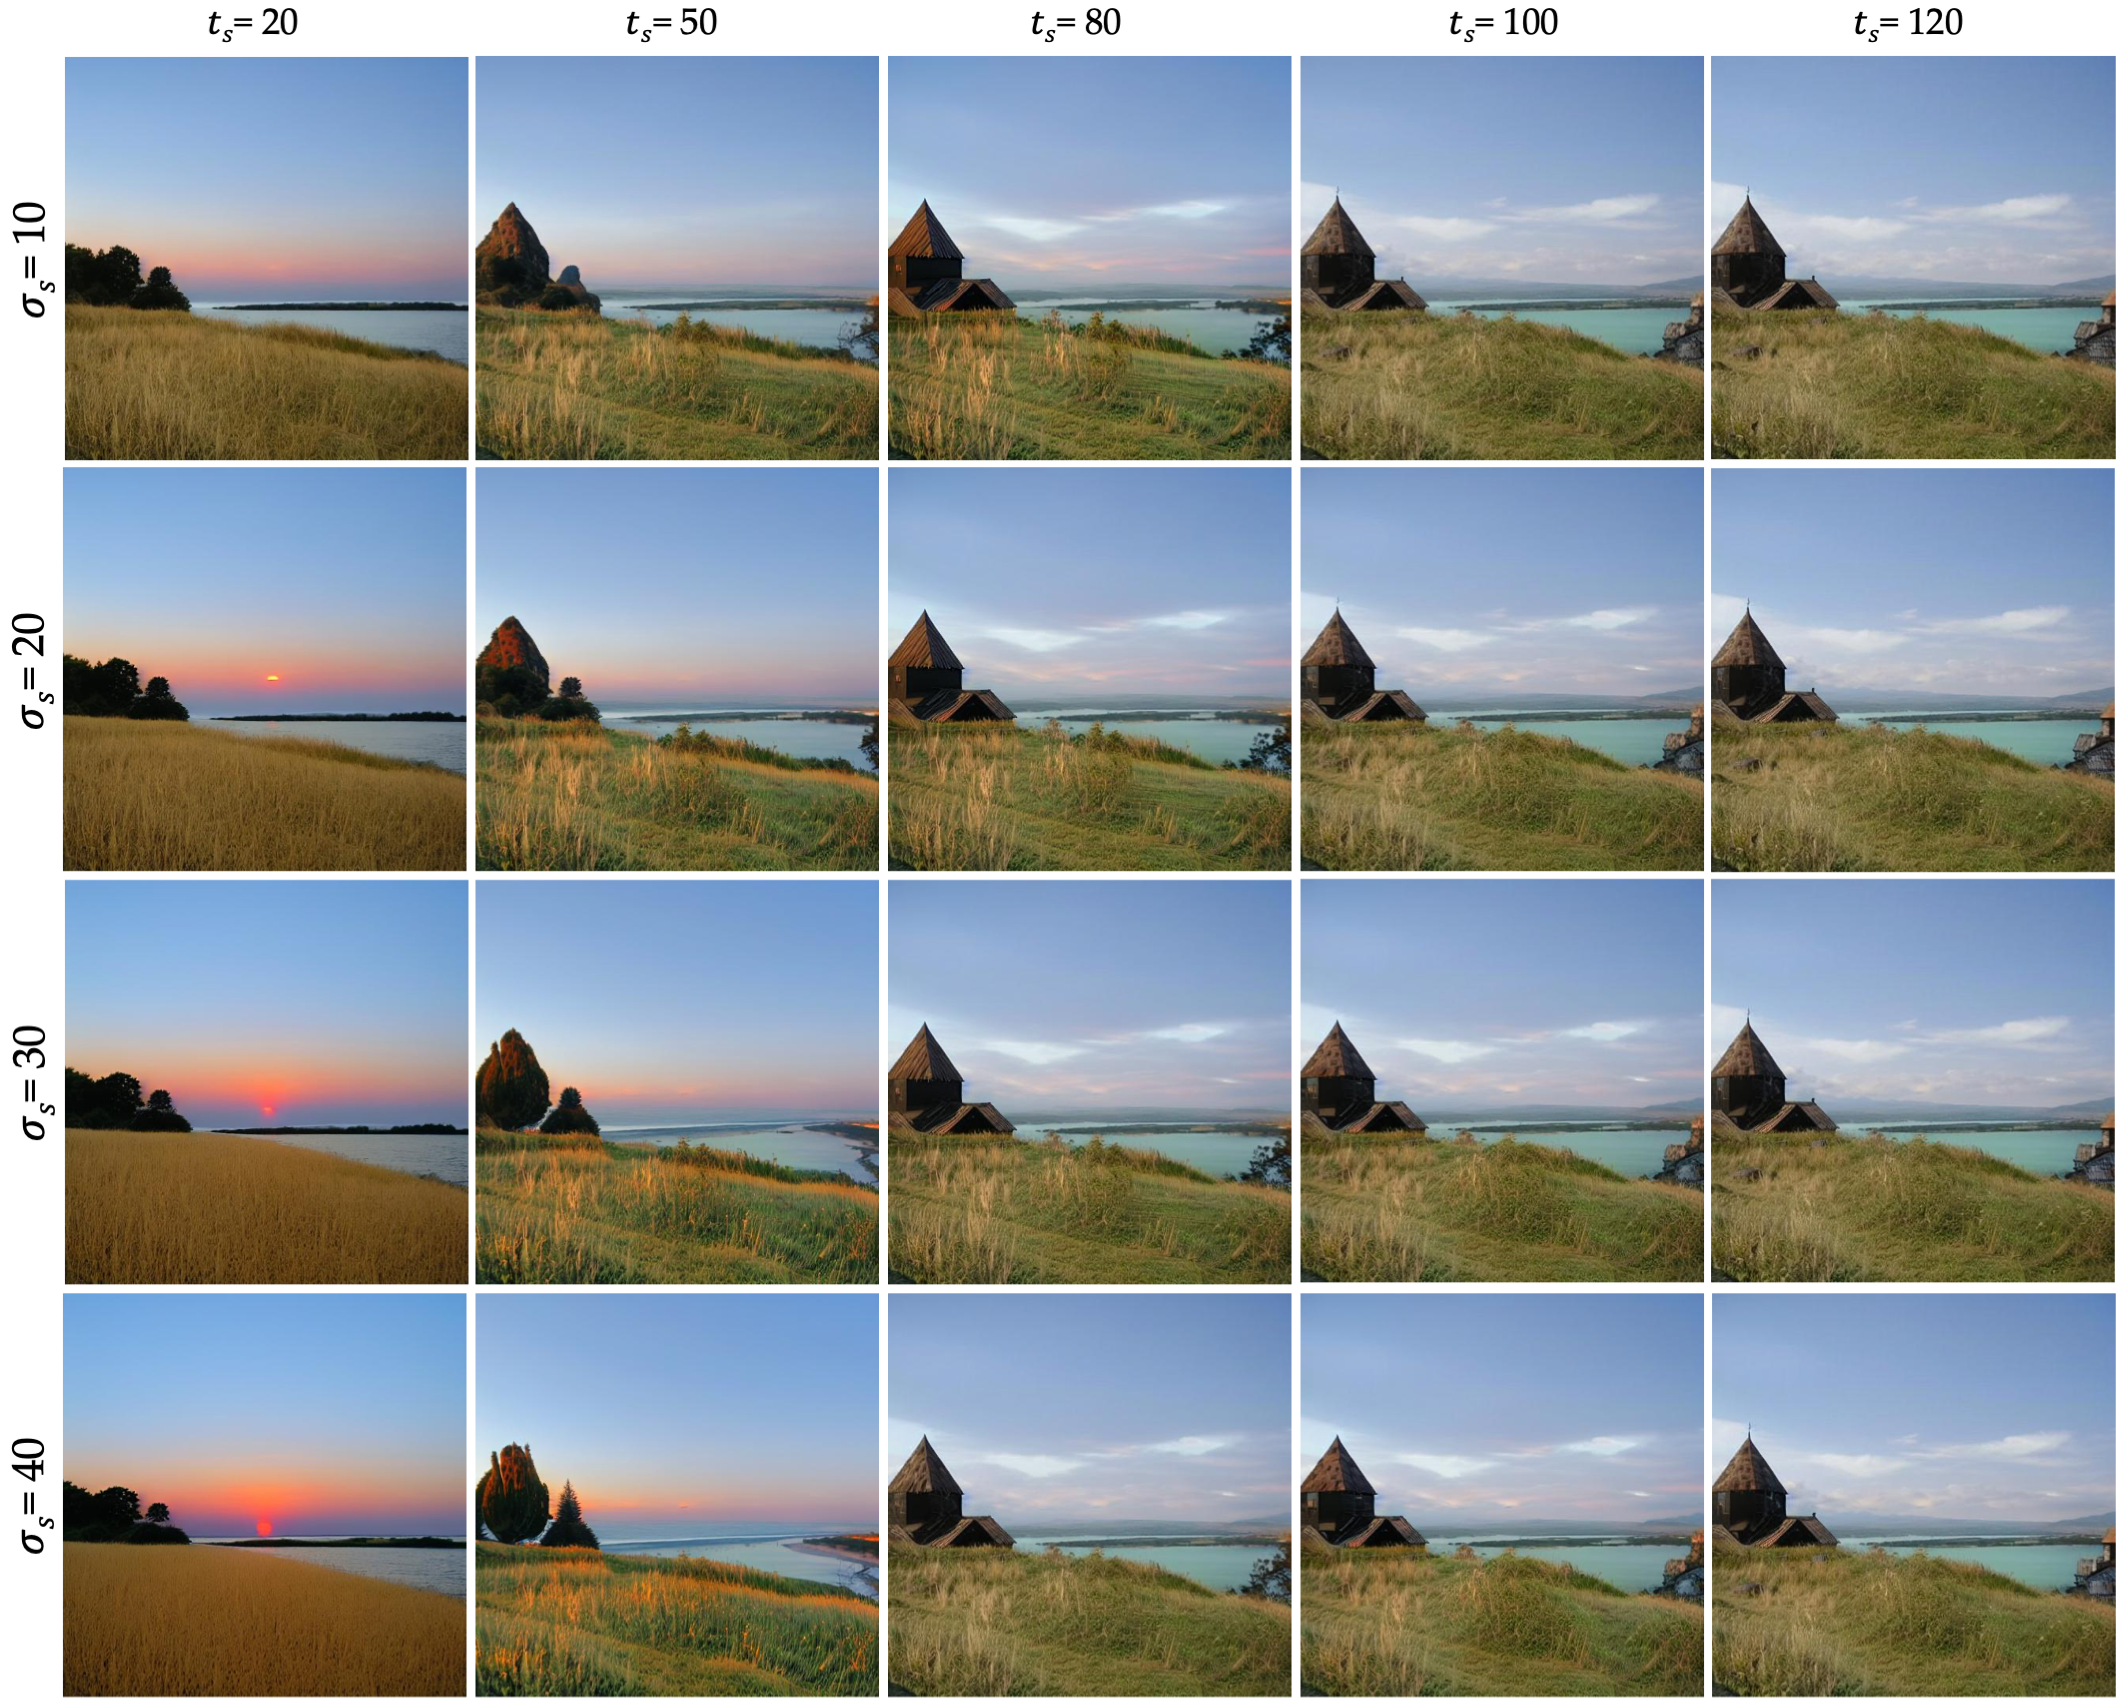
\includegraphics[width=\textwidth]{Chapters/zero-shot-tat-figs/grid-search.png}
  \caption{Grid search on DDIM inversion for the start step and the guidance scale. Here, the text prompt is "sunrise sunset".}
  \label{fig:zero-shot-grid-search}
\end{figure}

I ran an additional grid search on both parameters to find a balance between the text guidance and similarity to the input image. I experimented with $20, 50, 80, 100, 120$ for the start step out of the total number of 150 steps, and $10, 20, 30, 40$ for the guidance scale. Figure \ref{fig:zero-shot-grid-search} shows the grid search results for a test image, where we observe that increasing the guidance scale changes the appearance more strongly, whereas increasing the start step reduces the generation ability of the model.



\subsection{Qualitative comparison}
\paragraph{Baselines.} I also compare the finetuning and the zero-shot results with \citeauthor{laffont2014transient} \cite{laffont2014transient} and InstructPix2Pix \cite{brooks2023instructpix2pix} qualitatively. \citeauthor{laffont2014transient} \cite{laffont2014transient} learns the transforms from a pair of \textit{ Match - Target} images, as shown in the second and third columns. It has the disadvantage of requiring two additional images. On the other hand, InstructPix2Pix \cite{brooks2023instructpix2pix} is a diffusion-based model designed to edit images according to instructions. It is finetuned with a large dataset of image-target pairs along with their associated instructions. To adapt their model to our task, I convert the attributes to instructions by adding "make it" to the front of the adjective version of the attribute. For instance, if the prompt is initially "summer," then the InstructPix2Pix input becomes "make it sunny." Without this adjustment, I observed little to no changes in the input images.


 
 \begin{figure}[ht]
  \includegraphics[width=\textwidth]{Chapters/zero-shot-tat-figs/zeros-shot-qual-comp-updated.pdf}
  \caption{Qualitative comparison with the baseline methods on the test images of the Transient Attribute Dataset \cite{laffont2014transient}. Additional results can be found in Appendix \ref{TAT:add_res}.}
  \label{fig:zero-shot-comparison}
\end{figure}

Figure \ref{fig:zero-shot-comparison} shows that Zero-shot (right-most column) overall attains compelling results, comparable with InstructPix2Pix (fifth column). It maintains the core structures while transferring the target attributes to the input image. \citeauthor{laffont2014transient} \cite{laffont2014transient} can also accurately capture the transfer, but their edits remain limited to the \textit{Match - Target} pair, being unable to add some additional content, such as snow or raindrops. Both ControlNet (third column from the right) and Stable Diffusion (second from the right) are better capable of generating new content (clouds, snow, daylight, etc.). However, these models are less reliable in terms of content preservation. 



\section{Limitations and future work}
The grid search of the parameters in DDIM inversion is indeed sub-optimal, requiring manual labour for each image. Automatically optimising the parameter values based on a quantitative metric would be the future work of this project. Additionally, transient attributes usually rely on a continuous spectrum with less distinction between attributes as opposed to categories. In the future, I would like to explore the controllability of the transitions between the attributes, such as a slider interpolating appearances between two attributes, as done in the HyperBRDF work (BRDF editing, Section \ref{sec:brdf-editing}).

\section{Summary}

Transient attributes are the essence of the scene atmosphere, shaping its appearance dramatically in a natural way. Such changes to the appearance include highly complex patterns due to the coupled scene components, i.e., unknown illumination, reflectance, and geometry. In this chapter, I present highly accurate as well as creative transient attribute transfers captured by variants of pre-trained latent diffusion models. The observation that fine-tuning is costly and can overfit to a small dataset motivates me to utilise the pre-trained model as a prior in a zero-shot setting. The DDIM inversion offers a balance between the creation of new content and the preservation of the core features with a tweak of only two parameters (start step and guidance scale). This approach has the potential to advance scene appearance manipulations by eliminating the requirement of additional extensive datasets. 

%\TODO{explain fine-tuning GPU usage somewhere please}
% \begin{figure*}%[th]
%   \centering
%   \includegraphics[height=0.8\textheight, width=\linewidth,keepaspectratio]{Images/AdditionalResults_op2.pdf}
%   \caption{
%            Retouches reproduced by our algorithm based on single before-after pairs. }
%            \label{fig:AdditionalRes}%
% \end{figure*}

% \section{Appendices}
